\documentclass[
    linespread = 1.25
]{ctexart}
\pagestyle{plain}
\ctexset{
    section/format = \Large\bfseries\raggedright,
    section/number = {\chinese{section}、},
    section/aftername = {\enskip},
    abstractname = {\zihao{-2}摘\quad 要}
}

\usepackage[a4paper, lmargin=1in, rmargin=1in, tmargin=1in, bmargin=1in]{geometry}
\usepackage{amsmath}
\usepackage{booktabs}
\usepackage{graphicx}
\graphicspath{ {./fig} }

\usepackage{listings}
\usepackage{color}

\usepackage[sorting=none]{biblatex}
\addbibresource{LLMTuningReport.bib}

\definecolor{dkgreen}{rgb}{0,0.6,0}
\definecolor{gray}{rgb}{0.5,0.5,0.5}
\definecolor{mauve}{rgb}{0.58,0,0.82}

\lstset{
  frame=tb,
  language=Python,
  aboveskip=3mm,
  belowskip=3mm,
  showstringspaces=false,
  columns=flexible,
  basicstyle={\small\ttfamily},
  numbers=left,
  numberstyle=\tiny\color{gray},
  keywordstyle=\color{blue},
  commentstyle=\color{dkgreen},
  stringstyle=\color{mauve},
  breaklines=true,
  breakatwhitespace=true,
  tabsize=2
}

\usepackage[hidelinks]{hyperref}
\usepackage{caption}
\usepackage{subcaption}
\usepackage{siunitx}
\usepackage{algorithm2e}
\SetAlgoInsideSkip{bigskip}
\SetAlgorithmName{算法}{算法}{算法}
\RestyleAlgo{ruled}
\usepackage{multicol}
\usepackage{longtable}
\usepackage{tablefootnote}

\title{\zihao{2}\textbf{大数据创新实践实验报告}\\\zihao{3}\textbf{——多模态大模型LLaVA的微调}}
\author{\zihao{4}曹瀚文 \\\texttt{学号:210810503}
\and \zihao{4}岑畅 \\\texttt{学号:210810501}
\and \zihao{4}丁有罡 \\\texttt{学号:210810518}
\and \zihao{4}符永宣\\\texttt{学号:210810506}
\and \zihao{4}金文韬\\\texttt{学号:210810306}
\and \zihao{4}刘炎培\\\texttt{学号:210810510}
\and \zihao{4}刘梓涛\\\texttt{学号:210810513}
\and \zihao{4}彭珂\\\texttt{学号:210810508}
\and \zihao{4}王子霖\\\texttt{学号:210810522}
\and \zihao{4}文宇祥\\\texttt{学号:210810514}
}
\date{}

\begin{document}

\begin{titlepage}
  \newgeometry{top=1in,bottom=1in,right=0.75in,left=0.75in}
  \maketitle
  \vspace{0.2cm}
  \begin{abstract}
    \zihao{-4}
    \vspace{0.8cm}
    \linespread{1.25}
    本论文主要研究了空气质量、污染物水平及其与时空、气候因素的关系,并基于历史数据预测未来空气质量。论文首先对数据进行了预处理,包括数据描述、数据标准化、异常值及缺失值处理、极值值处理等步骤。接着,采用系统聚类方法对不同城市的污染物水平进行了潜在模式探索,通过均值和不同邻距离的聚类方法分析得出了系统聚类结果,并用因子分析的得分对其进行了解释。

    论文进一步探讨了空气质量与时空、气候因素的相关关系,应用多元线性回归模型和改进的多元线性回归模型,诊断模型结果并分析了气候因素与空气质量之间的相关性。此外,论文介绍并应用了广义线性模型,实现利用时空、气候因素对空气质量进行更加准确的预测。

    最后,论文利用SARIMA模型和GARCH模型,根据历史空气质量数据预测未来一段时间内的空气质量,以南昌市为例进行了实证研究。通过数据导入、探索性期性、参数确定、模型诊断及预测等步骤,详细展示了两种模型的应用过程和预测效果。

    本文不仅揭示了不同城市空气污染物可能存在的潜在模式,同时探究了空气质量与多种因素之间的复杂关系,也为空气质量的预测提供了有效的模型和方法,对城市环境管理、污染控制和空气质量的预报具有重要的参考价值。

    \vspace{1cm}
    \noindent\textbf{关键词:} 系统聚类\hspace{0.22cm} 因子分析\hspace{0.22cm} 多元线性回归\hspace{0.22cm} 广义线性模型\hspace{0.22cm} 时间序列分析
  \end{abstract}
\end{titlepage}

\tableofcontents
\newpage
\section{实验背景}
在当今人工智能和机器学习领域,预训练大规模语言模型(如GPT-4)已经展现出卓越的性能。然而,尽管这些模型在许多任务中表现优异,它们的通用性仍然可能无法满足特定应用场景的需求。因此,为了进一步提升模型在特定领域的效果,参数微调成为了一个关键的研究方向。通过微调,我们可以根据特定的数据集和任务需求对模型进行定制,使其在处理特定类型的输入时表现得更加精准和高效。这种方法不仅可以改善模型的预测能力,还能提升其对领域特定知识的理解和应用能力。为了实现最佳的微调效果,研究者们通常需要细致地调整模型的超参数,探索不同的优化策略,以便找到最适合特定应用场景的配置。

本次参数微调实验旨在通过自动驾驶数据集对LLaVA模型进行微调,以期提升该模型在自动驾驶领域的综合表现。同时,在该过程中我们希望探究微调过程中的关键影响因素,并采用多种方法评估微调效果。

% 本次实验选取的模型是开源的大语言模型LLaVA\cite{liu2023llava},该模型结合了语言模型和视觉模型,能够同时处理文本和图像输入,从而更好地理解和生成多模态信息,如图\ref{fig:LLaVA}所示。LLaVA通过大规模预训练学习到丰富的特征表示,并在特定任务中通过微调进一步优化性能,在自动驾驶、医疗影像分析、智能客服和内容创作等多个领域展现出广泛的应用前景和高效的推理性能。

% 本次实验将采用的是LoRA(Low-Rank Adaptation)参数微调算法\cite{hu2021loralowrankadaptationlarge},它是一种高效的参数微调方法,通过在预训练模型的权重矩阵上添加低秩分解来减少参数数量,如图\ref{fig:LoRA}所示。这种方法不仅显著降低了微调过程中所需的计算资源和存储空间,还能在保持模型性能的同时,快速适应新的任务和数据。LoRA通过只微调一小部分参数,使得大规模预训练模型的应用更加灵活和经济。

\begin{figure}[htbp]
  \centering
  \begin{minipage}[b]{0.6\textwidth}
    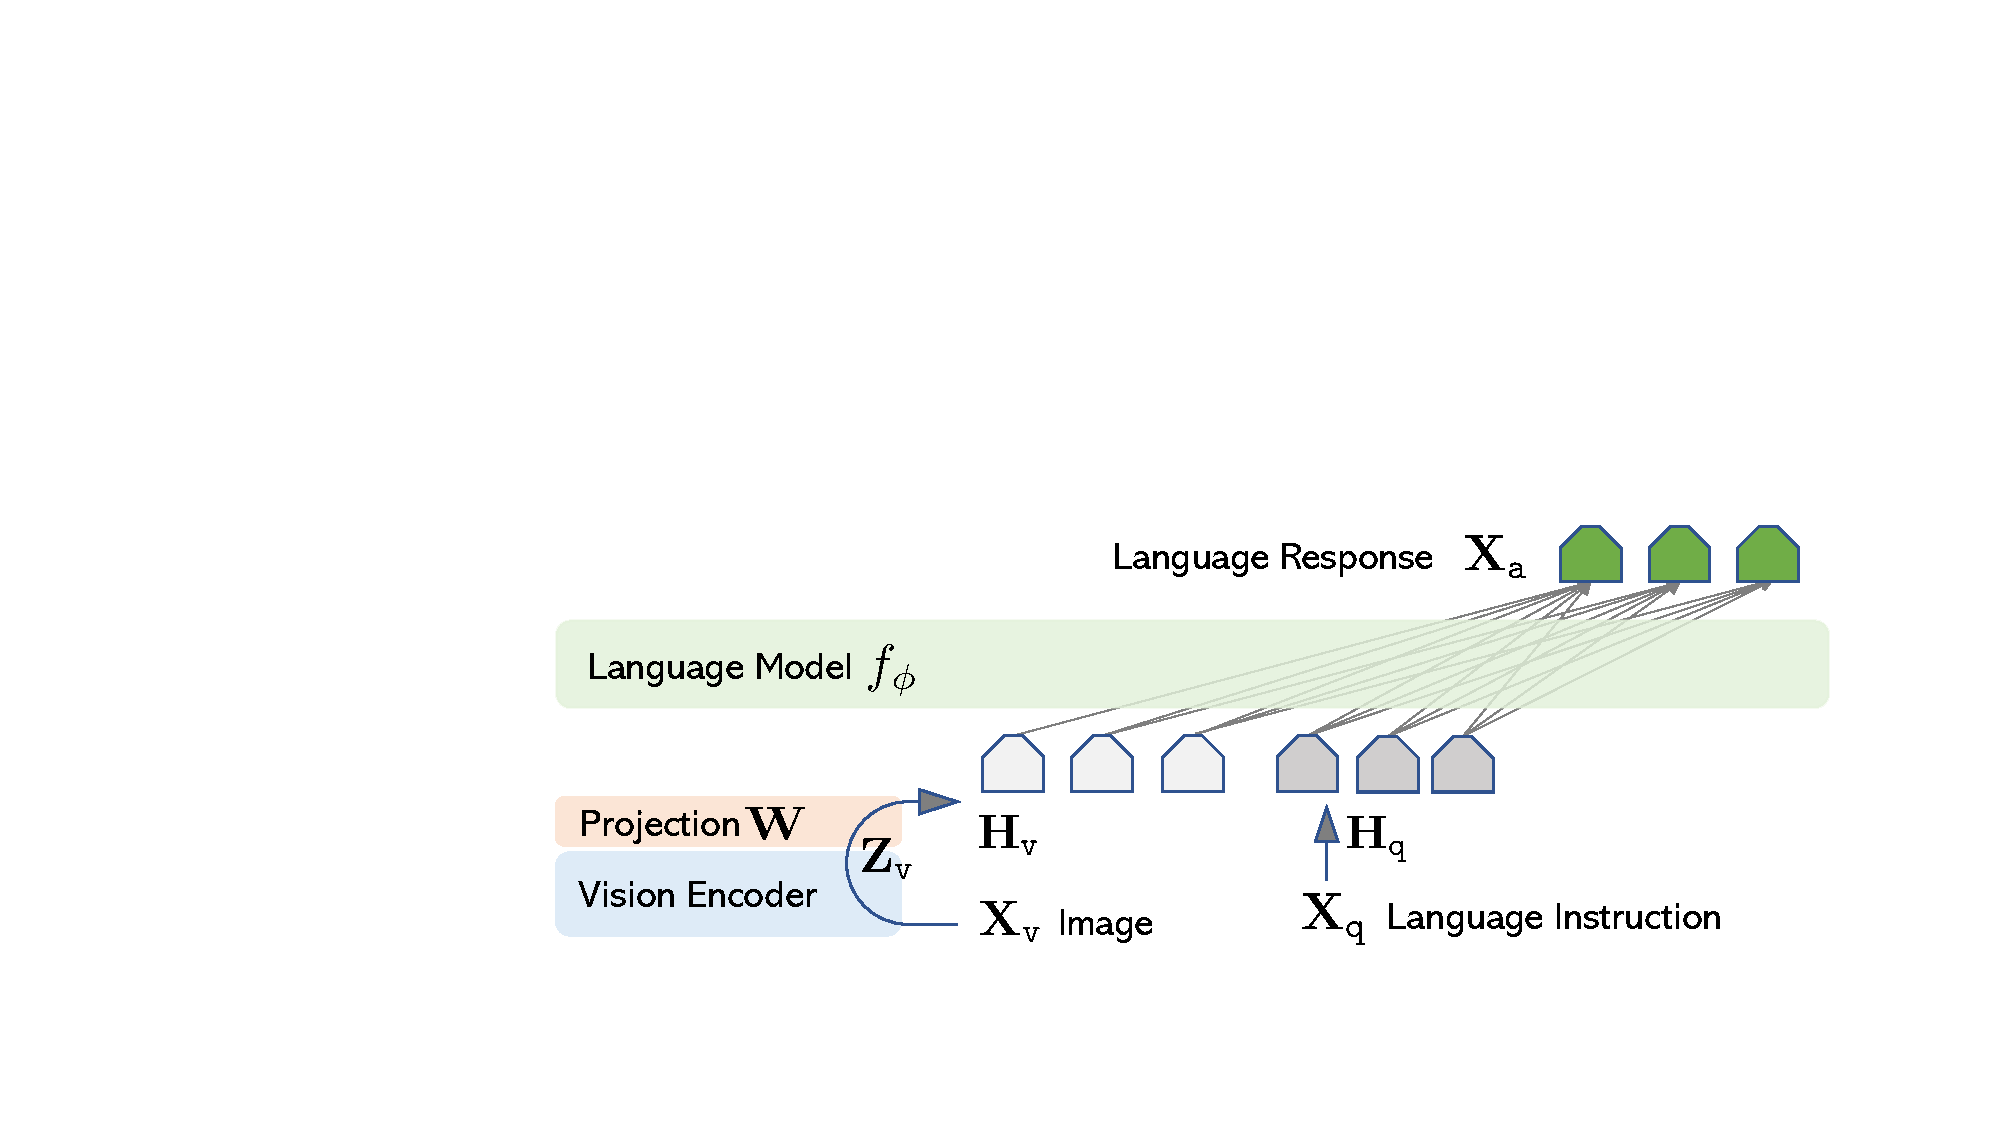
\includegraphics[width=\textwidth]{illu_llava.pdf}
    \caption{LLaVA模型架构}
    \label{fig:LLaVA}
  \end{minipage}
  \hfill
  \begin{minipage}[b]{0.25\textwidth}
    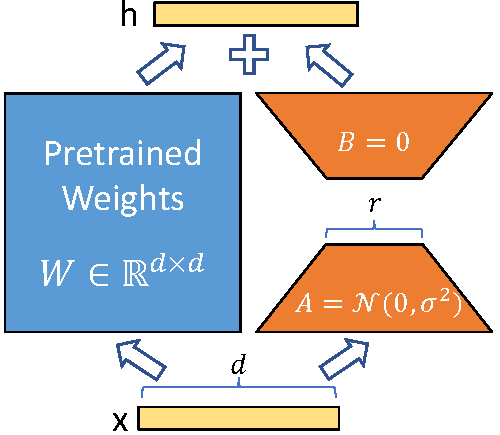
\includegraphics[width=\textwidth]{illu_lora.pdf}
    \caption{LoRA算法图解}
    \label{fig:LoRA}
  \end{minipage}
\end{figure}

% 本次实验在黎勃老师提供的Linux服务器平台上进行,通过SSH远程连接服务器进行实验。

\section{基于自动驾驶数据集的模型微调}

% \subsection{LoRA参数微调算法简介}

\subsection{使用LoRA算法和自动驾驶数据集对LLaVA模型作指令微调}

\subsection{实现微调模型的图形化界面}

\subsection{结论}

\section{探索影响微调效果的实验因素}

\subsection{探究训练周期对微调效果的影响}

\subsection{探究模型大小对微调效果的影响}

\subsection{结论}

\section{微调结果的分析与评估}

\subsection{使用维基百科数据集进行主观初步评估}

\subsection{计算微调模型的相关评价指标}

\subsection{使用CODA-LM数据集进行评估}
\subsubsection{数据集介绍}
\subsubsection{实验设计}
\subsubsection{评估结果}
\begin{table}[htbp]
  \centering
  \caption{Comparison of Different Methods}
  \small % 调整表格字体大小
  \renewcommand{\arraystretch}{1.2} % 调整行距
  \begin{tabular}{lccccccccccc}
    \toprule
    \textbf{Method}   & \textbf{General↑}   & \multicolumn{8}{c}{\textbf{Regional Perception↑}} & \textbf{Suggestion↑}                                                                                                                               \\
    \cmidrule(r){3-10}
                      & \textbf{Text-Score} & \textbf{ALL}                                      & \textbf{Vehicle}     & \textbf{VRU}   & \textbf{Sign}  & \textbf{Light} & \textbf{Cone}  & \textbf{Barrier} & \textbf{Other} & \textbf{Text-Score} \\
    \midrule
    MiniGPT-v2-7B     & 11.58               & 15.93                                             & 18.74                & 13.58          & 15.71          & 17.78          & 15.34          & 13.02            & 14.41          & 10.00               \\
    Shikra-7B         & 12.24               & 22.94                                             & 28.29                & 17.88          & 20.00          & 15.56          & 21.23          & 20.00            & 19.67          & 10.20               \\
    LLaVA1.5-7B       & 19.30               & 42.06                                             & 46.67                & 38.47          & 39.14          & 48.89          & 50.83          & 30.93            & 33.82          & 23.16               \\
    Qwen-VL-Chat-7B   & 18.22               & 26.62                                             & 35.48                & 24.16          & 20.86          & 23.33          & 19.61          & 17.56            & 25.86          & 22.06               \\
    MiniCPM-V-2.5-8B  & 41.12               & 57.20                                             & 61.91                & 54.82          & 59.43          & 46.67          & 66.57          & 35.35            & 58.75          & 48.48               \\
    \midrule
    LLaVA1.5-13B      & 24.54               & 42.41                                             & 53.62                & 36.79          & 33.71          & 46.67          & 41.27          & 30.41            & 33.82          & 27.90               \\
    LLaVA-NeXT-13B    & 29.86               & 53.63                                             & 55.51                & 47.08          & 54.00          & 60.00          & 70.34          & 40.47            & 46.45          & 31.92               \\
    InternVL-V1-5-20B & 38.38               & 61.53                                             & 63.77                & 53.14          & 50.57          & 57.78          & 80.34          & 46.86            & 57.11          & 41.18               \\
    \midrule
    Gemini-Pro        & 25.24               & 51.38                                             & 49.03                & 42.77          & 37.43          & 42.22          & 69.56          & 45.70            & 51.32          & 27.40               \\
    GPT-4V            & \textbf{57.50}      & 56.26                                             & 60.89                & 40.58          & 49.43          & 54.44          & 66.08          & 50.17            & 53.16          & \textbf{63.30}      \\
    \midrule
    CODA-VLM (ours)   & \textbf{55.04}      & \textbf{77.68}                                    & \textbf{78.79}       & \textbf{73.80} & \textbf{64.86} & \textbf{73.33} & \textbf{86.18} & \textbf{78.72}   & \textbf{68.75} & \textbf{58.14}      \\
    \bottomrule
  \end{tabular}
\end{table}

\subsection{结论}

\section{实验结论}

\appendix
\newpage
\section*{参考文献}
\addcontentsline{toc}{section}{参考文献}
\printbibliography[heading=none]
% \noindent
% [1] 乐东明,王文浚,王颖,等. 2020—2022年咸宁市臭氧污染气象特征及成因分析[J].黑龙江环境通报, 2024, 37(05):30-32.

% \noindent
% [2] 李高荣,吴密霞. 多元统计分析[M]. 北京:科学出版社, 2021

% \noindent
% [3] John A. Rice. Mathematical Statistics and Data Analysis[M]. Boston: Cengage Learning, 2006

% \noindent
% [4] 何书元. 应用时间序列分析[M]. 北京:北京大学出版社, 2003

\newpage
\section*{附录:实验日志与心得}
\addcontentsline{toc}{section}{附录:实验日志与心得}

\end{document}

